\chapter{INTRODUCTION}
\graphicspath{{Chapter1/}}

\section{Background}
Chest X-ray or chest radiography has been for a long time a widely used and cost-effective imaging technique for the diagnosis and monitoring of thoracic diseases, which include diseases like pneumonia, TB, edema, lung nodules, etc. The major reasons behind this are the accessibility, low radiation exposure (so low risk), and non-invasive nature of this technique. However, the study of these radiographs requires expertise, and the growing volume of imaging studies has created a demand that is difficult to meet considering the limited availability of trained radiologists; therefore, there is a need for automated and computer-aided diagnostic (CAD) systems.
\newline
Although recent advancements in AI, specifically Deep Learning, have achieved significant success in medical image analysis, to be more precise, Convolutional Neural Networks (CNNs) and recent Vision Transformer (ViT) models have achieved promising performance in disease classification, abnormality detection, and segmentation. Despite these advancements, several problems and challenges still remain, such as relying heavily on supervised learning, i.e., large volumes of labeled data. Another problem is that many such models operate as black boxes, i.e., interpretability is too low pertaining to the spatial grounding and extent of abnormalities, and in clinical settings, interpretability is important and highly appreciated.


\section{Problem Statement}

Although deep learning models have achieved promising results in multi label chest X-ray classification, most existing systems:

\begin{itemize}
    \item Operate as black-box classifiers.
    \item Do not provide spatial localization of detected pathologies.
    \item Do not generate clinically structured radiology reports.
    \item Lack explainability and fine-grained disease-region alignment.
\end{itemize}

There is therefore a need for an end-to-end, explainable, and multimodal AI system that can:

\begin{enumerate}
    \item Learn robust visual representations from large-scale chest X-ray data.
    \item Perform multi label disease classification.
    \item Localize pathological regions.
    \item Provide interpretable evidence for predictions.
    \item Generate structured radiology-style reports.
\end{enumerate}

\section{Formal Problem Definition}

\subsection{Input}

For each patient case, the system receives:

\begin{enumerate}
    \item A chest X-ray image:
\[
X \in \mathbb{R}^{H \times W \times 3}
\]

\begin{figure}[H]
    \centering
    
    % --- Three X-rays in a single row ---
    \begin{subfigure}{0.32\textwidth}
        \centering
        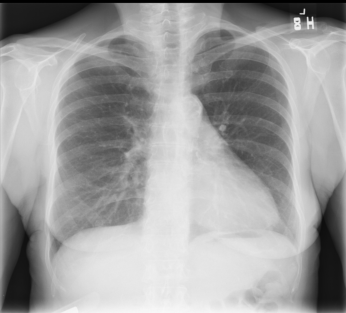
\includegraphics[width=\linewidth,height=0.18\textheight,keepaspectratio]{xray1.png}
        \caption{Sample X-ray 1}
    \end{subfigure}
    \hfill
    \begin{subfigure}{0.32\textwidth}
        \centering
        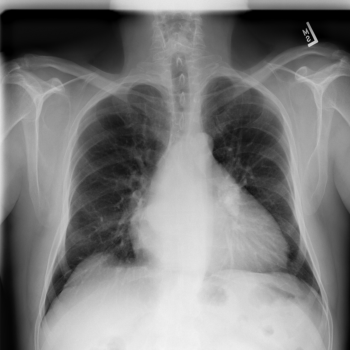
\includegraphics[width=\linewidth,height=0.18\textheight,keepaspectratio]{xray2.png}
        \caption{Sample X-ray 2}
    \end{subfigure}
    \hfill
    \begin{subfigure}{0.32\textwidth}
        \centering
        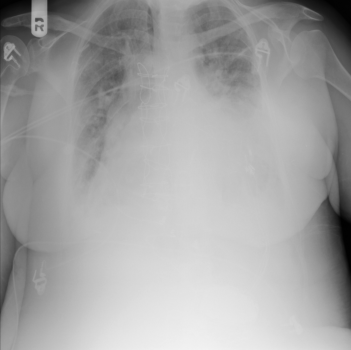
\includegraphics[width=\linewidth,height=0.18\textheight,keepaspectratio]{xray3.png}
        \caption{Sample X-ray 3}
    \end{subfigure}

    \vspace{0.3cm}

    % --- Metadata dataframe image below ---
    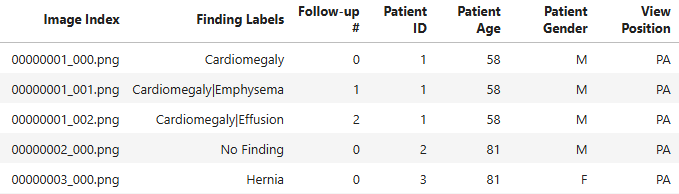
\includegraphics[width=0.8\textwidth,height=0.25\textheight,keepaspectratio]{metadata_dataframe.png}
    
    \caption{Example chest X-ray samples (top) and corresponding patient metadata (bottom).}
    \label{fig:input_samples}
\end{figure}
    \item Patient metadata:
    \[
    M = \{\text{Age}, \text{Gender}, \text{View Position}\}
    \]

    \item (During training) Ground-truth multi-label disease annotations:
    \[
    Y \in \{0,1\}^{C}
    \]
    where \( C \) denotes the number of disease classes.

    \item (Optionally during training) Bounding box annotations for disease localization.

    \item (Optionally during training) Corresponding radiology reports for text generation.
\end{enumerate}
\subsection{Output}

The system is required to produce:

\begin{enumerate}
    \item Multi-label disease prediction probabilities:
    \[
    \hat{Y} \in [0,1]^{C}
    \]

    \item Binary disease decisions after thresholding:
    \[
    \tilde{Y} \in \{0,1\}^{C}
    \]

    \item Predicted bounding boxes
    Let the input image be defined as:

\[
X \in \mathbb{R}^{H \times W \times 3}
\]

where \(H\) and \(W\) denote the height and width of the image.

For each disease class \(c \in \{1, 2, \dots, C\}\), the model predicts at most one bounding box corresponding to the detected pathological region.

The predicted bounding box for class \(c\) is defined as:

\[
\hat{b}_c = \left( x_c^{(1)}, y_c^{(1)}, x_c^{(2)}, y_c^{(2)} \right)
\]

such that:

\[
0 \leq x_c^{(1)} < x_c^{(2)} \leq W
\]

\[
0 \leq y_c^{(1)} < y_c^{(2)} \leq H
\]

where:

\begin{itemize}
    \item \( (x_c^{(1)}, y_c^{(1)}) \) denotes the top-left corner,
    \item \( (x_c^{(2)}, y_c^{(2)}) \) denotes the bottom-right corner,
    \item Coordinates are expressed in the same spatial reference frame as the input image.
\end{itemize}

    
    \item A structured radiology report:
    \[
    \hat{R} = \text{Generated textual report describing findings and impressions}
    \]
\end{enumerate}

\section{Motivation}

The global healthcare system continues to face an increasing burden of pulmonary diseases such as pneumonia, pneumothorax, edema, etc. Among the widely used cost-effective diagnostic tools for detecting such problems and diseases is the chest X-ray (CXR). Hospitals generate thousands of chest radiographs daily, especially at tertiary centers and emergency departments. But again, the issue is that accurate interpretation of these images requires trained radiologists, so in situations where human resources are scarce, backlogs are created. This leads to late diagnosis, which may even prove fatal, so obviously there is a need for rapid and reliable chest X-ray interpretation.

The primary motivation for pursuing this project is to develop a unified, explainable chest X-ray analysis system that leverages the abilities of SSL (Self-Supervised Learning), multi-label classification, bounding box localization, and automated report generation to bridge the gap between simple image-level prediction and clinically useful results.

Another key motivation is the need to address the limitations of supervised learning in medical imaging systems. Labeled datasets suffer from issues of class imbalance and a scarcity of abnormalities in the dataset, which makes it difficult to train a model to learn useful features.

There has also been a growing need to produce AI models in medical and healthcare systems, especially ones that have interpretability and can ground predictions spatially. This is because having explainability in a system allows the HiTL (Human in the Loop) to check if the predictions are right and whether the reason for those predictions is also right. This also helps in training a model based on feedback (Reinforcement Learning).

\section{Objectives}
\subsection{Primary Objectives}
The primary objective of this project is to enhance the classification capability and performance on chest X-rays using advanced representational learning and optimization strategies.
\begin{enumerate}
\item The objective is to improve the classification performance (AUC and F1 are the metrics of concern) using architectures like EfficientNet or Vision Transformers (like Swin and DINO).
\item To integrate SSL (Self-Supervised Learning) as a pretraining step before supervised learning so that the model can learn robust anatomical features from unlabeled data.
\item To study the impact of introducing SSL compared to just using common deep learning models for better generalization ability.
\item To analyze the model's robustness by calculating per-class AUC and macro/micro F1 scores.
\item To compare various architectures like EfficientNet, DenseNet, and Swin/DINO to determine the best feature extractor for the task.
\end{enumerate}
\subsection{Secondary Objectives}
The secondary objective is to design an end-to-end pipeline that extends beyond just classification to a complete chest radiology system.

\begin{enumerate}
\item To implement bounding box localization of diseases; this ensures spatial grounding.
\item To perform segmentation of the lung region to identify regions within the lungs for radiology report generation and spatial grounding.
\item To develop a radiology report generation module that can use structured outputs to generate logical and relevant textual reports.
\end{enumerate}

\subsection{Tertiary Objectives}
To design a complete GUI and backend framework and deploy the solution for public usage with necessary caution, permissions, and licenses.